\section{Styrhandske}

\begin{figure}[H]
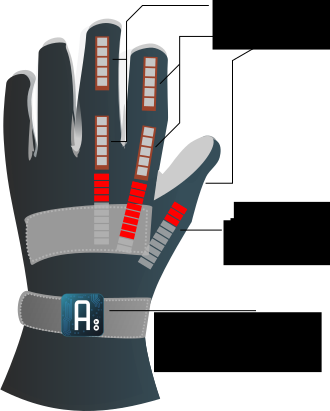
\includegraphics[height=0.5\textheight]{img/kontrollhandske}
\caption{Konceptskiss över styrhandsken}
\end{figure}

För att intuitivt reglera robothanden används en vanlig handske som användaren bär på sin hand. På tumme, långfinger och pekfinger finns det två flexsensorer vardera. Flexsensorerna ändrar resistans beroende på hur böjda de är, vilket leder till  

 vilket används för att översätta de tre fingrarnas läge till önskvärda vinklar för robothandens fingrar. När resistansen ändras, 

 ändrad resistans $\to$ ändrad spänning $\to$ spänningen normaliseras mot fingrarnas referens $\to$ önskvärd vinkel skickas till robothanden


% För att reglera robothanden används en reglerhandske som användaren har på sin hand, detta ger en intuitivt reglering (se figur). På tumme, pekfinger och långfinger på handsken sitter två flexsensorer var som följer användarens hand och ändrar resistans beroende på hur mycket de böjs. Denna resistansförändring använder man som insignal till mikrokontrollen som sitter på reglerhandsken, som i sin tur skickar styrsignaler till mikrokontrollen på robothanden. Se \ref{sec:mikro}. 

% Handsken är gjord av textil och flexsensorerna är insydda i små påsar som underlättar montering av sensorerna på handsken. (Se figur)
% (Bild på handsken)  
\section{Trådlös kommunikation}
\section{Signalbehandling}
\section{Mikrokontroller}
\label{sec:mikro}
info om våra microcontroller. Bluetooth moduelerna och hur det programmerats samt hur det fungerar.
\section{Elektriska kretsar}
\begin{figure}[H]
\includegraphics[height=0.5\textheight]{img/schemahandske}
\caption{Kopplingsschema för styr/regler-handsken.}
\end{figure}
\begin{figure}[H]
\includegraphics[height=0.5\textheight]{img/schemahand}
\caption{Kopplingsschema för robothanden.}
\end{figure}


Figur \ref{} visar hur styrhandsken är kopplad. Komponenterna är lödda på ett experimentkort.

\section{Algoritmer}
Här presenteras de styralgortimter som bestämmer hur handen beter sig när den följer användarens input samt identifierar och greppar objekt. 
\subsection{Objektidentifiering}
\begin{figure}[H]
EN BILD SOM FÖRKLARAR DETTA, SAMT VILKA OBJEKT VI VALT ATT identifierar och hur vi gör det...
\caption{Beskrivning}
\end{figure}
Antaganden: Servona står i önskat läge, det vill säga tidsfördröjningen som uppstår då servona skall vrida sig från godtycklig position till den önskade antags vara så liten vid normalt användande att den kan försummas. Då ingen mätning av servonas verkliga position görs, är den enda informationen om fingrarnas lägen det önskade servoläget. 

FIXA FLÖDESSSCHEMA OCH ETT ARDUINO PROGRAM Känner av tryck (över visst gränsvärde) på tumme och motstående finger->, lagrar användarens input läge då detta inträffar ( för att när användaren går utanför detta igen (öppnar sin hand) så skall handen återgår till att följa användaren) -> beräknar avståndet mellan sensorerna-> checkar av avståndet mot en lista av fördefinerade objekt som innehåller , storlek och önskat trycksensorvärde med en +/-tolerans för att inte handen ska stå och flippa som en tok för att uppnå EXAKT rätt värde-> TADAA!!-> när användaren öppnar sina fingrar utanför "kontaktläget" följer handen efter igen...
Mer teksti
